\documentclass[14pt]{article}
\usepackage[frenchb]{babel}
\usepackage[utf8]{inputenc}
\usepackage[T1]{fontenc}
\usepackage{glossaries}
\usepackage{graphicx}
\usepackage{float}
\usepackage{geometry}
\usepackage{fancyhdr}
\usepackage{xcolor}
\usepackage{listings}
 \usepackage{amsmath}
 \usepackage{textcomp} 
 \usepackage{chemist}
\usepackage{multicol} 
\usepackage{steinmetz}
\usepackage{colortbl}
\usepackage[hidelinks]{hyperref}
\usepackage{titlesec}
\usepackage{multirow}
\usepackage{amsfonts}
\usepackage{amssymb}
\usepackage{gensymb}
\usepackage{csquotes}
\usepackage{wrapfig}
\usepackage{pgfplots}
\usepackage{cancel}
 \usepackage{subcaption}
 \usepackage[final]{pdfpages}

\titleclass{\subsubsubsection}{straight}[\subsection]

\newcounter{subsubsubsection}[subsubsection]
\renewcommand\thesubsubsubsection{\thesubsubsection.\arabic{subsubsubsection}}
\renewcommand\theparagraph{\thesubsubsubsection.\arabic{paragraph}} % optional; useful if paragraphs are to be numbered

\titleformat{\subsubsubsection}
  {\normalfont\normalsize\bfseries}{\thesubsubsubsection}{1em}{}
\titlespacing*{\subsubsubsection}
{0pt}{3.25ex plus 1ex minus .2ex}{1.5ex plus .2ex}

\makeatletter
\renewcommand\paragraph{\@startsection{paragraph}{5}{\z@}%
  {3.25ex \@plus1ex \@minus.2ex}%
  {-1em}%
  {\normalfont\normalsize\bfseries}}
\renewcommand\subparagraph{\@startsection{subparagraph}{6}{\parindent}%
  {3.25ex \@plus1ex \@minus .2ex}%
  {-1em}%
  {\normalfont\normalsize\bfseries}}
\def\toclevel@subsubsubsection{4}
\def\toclevel@paragraph{5}
\def\toclevel@paragraph{6}
\def\l@subsubsubsection{\@dottedtocline{4}{7em}{4em}}
\def\l@paragraph{\@dottedtocline{5}{10em}{5em}}
\def\l@subparagraph{\@dottedtocline{6}{14em}{6em}}
\makeatother
\renewcommand{\baselinestretch}{1.1}
\setcounter{secnumdepth}{4}
\setcounter{tocdepth}{4}
\newcommand{\tens}[1]{\underline{\underline{#1}}}
\newcommand\bbox[1]{%
  \fbox{\begin{minipage}{0.9\textwidth}#1\end{minipage}}}
 \newcommand{\HRule}{\rule{\linewidth}{0.5mm}}
  
\newcommand{\RomanNumeralCaps}[1]
    {\MakeUppercase{\romannumeral #1}}
    
    \setlength{\parindent}{8 mm}
 
 \geometry{
a4paper,
left=20mm,
right=20mm,
top=20mm,
}
\pagestyle{fancy}
\lhead{}
\chead{}
\rhead{\textsc{Analyse du problème}}
\lfoot{\textsc{Made with \LaTeX}}
\rfoot{\thepage}
 
\newlength{\larg}
\setlength{\larg}{14.5cm}
 \graphicspath{{Image}}
\graphicspath{{C:/Users/Morar/Desktop/HE2B/ISIB/Prototypage/Latex/Image}}

\makeglossaries

%\newglossaryentry{bancTest}
%{
%	name = banc de test,
%	description={test d'un objet/produit afin de le caractériser, il s'agit de connaitre sa durée de vie, sa résistance, comment prévoir son obsolescence,...}
%}
 
% La commande \title... bien chargée ! 
\pgfplotsset{compat=1.18}

\begin{document}

%%%%%%%%%%%%%%%%%%%%%%%%%%%%%%%%%% PAGE_DE_GARDE %%%%%%%%%%%%%%%%%%%%%%%%%%
\begin{center}
%%%
\begin{minipage}{0.48\textwidth} \begin{flushleft}

\includegraphics[scale = 1.7]{Image/HE2B.png}
\end{flushleft}\end{minipage}
\begin{minipage}{0.48\textwidth} \begin{flushright}

\includegraphics[scale = 0.25]{Image/ISIB.png}
\end{flushright}\end{minipage}\\[1cm]
%%%	
\textsc{\LARGE Institut Supérieur \\ Industriel de Bruxelles\\ \vspace{10px} \huge I.S.I.B.}\\[1cm]	
\textsc{\large HE2B - orientation ingénieur industriel \\ en 
Électronique }\\[1cm]
%%%
\begin{minipage}{0.9\textwidth} 
\begin{center}
%%%
\textsc{\large $1^{\text{ère}}$ Année Master}
\end{center}
\end{minipage}\\[0.5cm]
%%%
\vspace*{0.5cm}
%%%
\HRule \\[0.5cm]
%%%
{\huge \bfseries Prototypage\\ 
\vspace{10px} Analyse du problème
}\\[0.4cm]
%%%
\HRule \\[1.5cm]
%%%
\begin{minipage}{0.46\textwidth}						
\begin{flushleft} \large
%%%
\textit{Auteur:}\\
Leonardo Rafael \bsc{Mora}
\end{flushleft}	
\end{minipage}		
%%%
\begin{minipage}{0.52\textwidth}		
\vspace{-0.5cm}											%%%
\begin{flushright} \large
%%%
\textit{Professeur :} \\	

G. \bsc{Le Vaillant}
%%%
\end{flushright}
%%%
\end{minipage}	
\vspace*{1cm}
%%%
\vspace{2cm}

\begin{center}									
{\large \today}										
\end{center}

\end{center}	
\thispagestyle{empty}
\newpage		

\thispagestyle{empty}
\tableofcontents

\thispagestyle{empty}
\listoffigures
%\listoftables
\newpage

\setcounter{page}{1}
\clearpage

\section{Remise en contexte}

Dans le cadre du cours, nous devons effectuer un projet qui consiste à l'élaboration de deux manettes gyroscopique.
Ces manettes utilisent un module d'acceleration 3DoF et un capteur de force chacune. Ils permettent donc l'envois de données suivantes:
\begin{itemize}
\item Pitch est la rotation autour de l'axe X (verticale).
\item Roll est la rotation autour de l'axe Y (transversale).
\item Weight est le poids ou la force.
\end{itemize}

\begin{figure}[H]
    \centering
    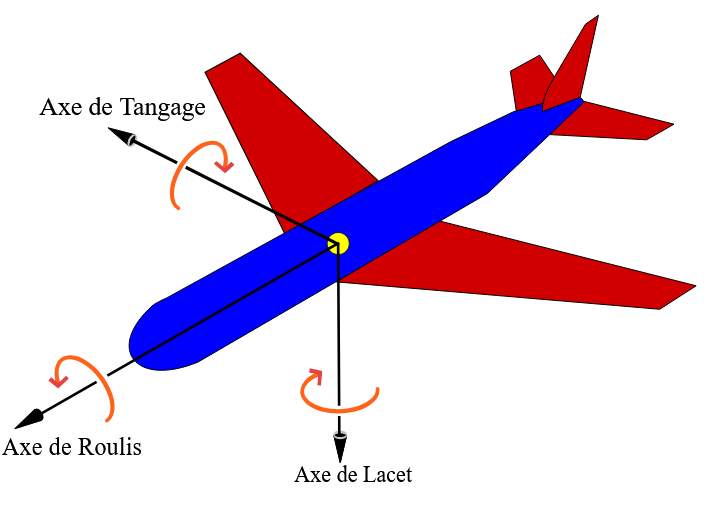
\includegraphics[width=0.7\textwidth]{Image/Yaw_Axis_Corrected.png}
    \caption{Position des 3 axes}
\end{figure}

Pitch et Roll sont basés sur les données d'accélération du capteur MMA8452Q et Weight est basé sur le capteur HX711.

Les deux manettes utilisent un Teensy LC avec le protocole HID. Ce protocole permet d'échanger des informations à grande vitesse.

Ce protocole permet de définir l'utilisation du device, le contenu de chaque valeur ainsi que des informations supplémentaires.
\newpage

\section{Explication du problème}
Lors du codage du Teensy, nous avons utilisé le protocole HID pour Joystick. Il permet l'ajout de divers données dont les axes X, Y, Z et 2 sliders.

\begin{figure}[H]
    \centering
    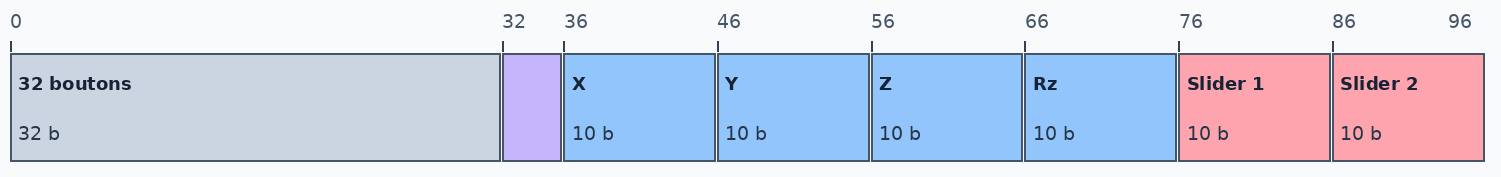
\includegraphics[width=\textwidth]{Image/trame_ancien_joystick.png}
    \caption{Trame de données HID Joystick}
\end{figure}

Le problème se trouve dans le positionnement des données pour des mêmes types de données et la librairie de base de Unity permettant de les utiliser.

Une fois que nous avons configuré, nous avons testé les manettes avec un utilitaire de Windows afin de voir les données reçues et voir la bonne configuration du HID, nous avons également développer une vue avec 2 cube afin de voir les manettes en action, c'est à ce moment là que nous avons observé que les capteurs de forces mises dans les sliders avaient un problème, la librairie ne reconnaissait qu'un seul slider alors que deux étaient bien configurés.

Le problème déduit est le mauvais développement de la librairie (rudimentaire) de Unity, un problème se trouvant également sur Linux.\\
En général les développeurs utilisent les informations envoyé par le device pour ensuite extraire les données. Lors d'envoie de trames, une trame contenant une table descriptive du device et de ses entrées est envoyé en premier, et ensuite nous recevons/envoyons les données.
\newpage

\section{Solutions proposées}

Plusieurs solutions peuvent le contourner:
\begin{itemize}
\item Utiliser au lieu de deux sliders, l'entrée Rz et un slider.\\ Pour un développeur il pourrait croire que ce soit de vrai entrées X, Y, Z et Rz alors que ce sont des roll, pitch et force.
\item Modifier une entrée de table HID par Dial, cette déclaration est utilisé notamment lors de problèmes de reonnaissance distinctes tels que les sliders sur Linux.
\item Utiliser une configuration de Joystick avec plus d'entrées, et utiliser des entrées analogiques différentes au choix.\\ Pour un développeur, les données définies et les données reçues peuvent porter à confusion, de plus la trame sera beaucoup trop long car il y aura beaucoup plus d'entrées.
\item Créer sa propre table HID avec des entrées spécifique à Roll, Pitch et Weight. Les données déclarées seront les vraies données reçues.\\
C'est plus compliqué à développer car nous devons définir la table HID et la fonction de trame à envoyer, mais elle respectera complètement les normes HID.
\end{itemize}


La solution actuellement étudiée est la création de sa propre table HID.\\
Elle sera basée sur cette trame là:

\begin{figure}[H]
    \centering
    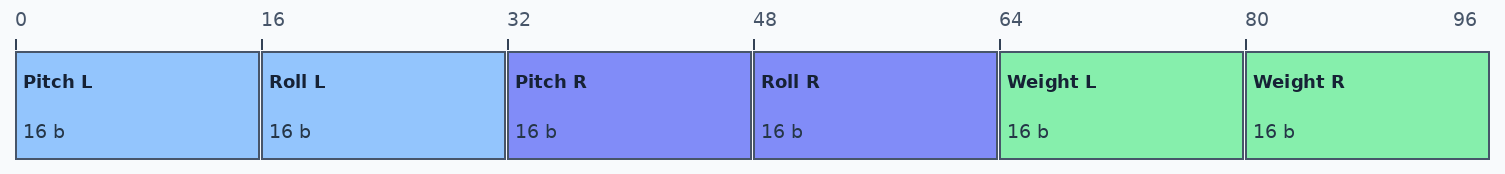
\includegraphics[width=\textwidth]{Image/trame_nouveau_controller.png}
    \caption{Trame de données HID Multi-axis Controller}
\end{figure}

Nous nous basons sur le document HID Usage Tables for Universal Serial Bus (USB) de USB Implementers Forum, qui définit les normes de HID et nous utiliserons les différents ID pour créer notre table.

\begin{table}[H]
\centering
\begin{tabular}{|c|c|c|}
  \hline
   Name  & Type  & Usage ID [HEX]\\
  \hline
    Multi-axis Controller & Collection application & 0x08\\
  \hline
    Pitch Forward/Backward & Dynamic Value & 0x22\\
  \hline
    Roll Right/Left & Dynamic Value & 0x23\\
  \hline
    Data Weight & Dynamic Value & 0x40\\
  \hline
\end{tabular}
\caption{Table HID Multi-axis Controller}
\end{table}
\footnotetext{Collection Application permet de définir l'usage et les fonctions du device.}

Cela permettra d'utiliser une table selon les bonnes normes de HID.
Si l'utilisation des Data weight cote à cote dans la trame pose problème, nous pouvons en remplacer une entrée par Data Scaling (0x41) afin de les différencier.


\newpage	







\clearpage

 
\end{document}
